\section{Rocket Attitude Module}

\subsection{Rocket Attitude Display Module}
The Rocket Attitude display takes in gyro data and a 3D model. It renders this 3D model, and then uses the received gyro data to alter the orientation of the model to match that of the live rocket.

\subsubsection{Model Storage}
There will be an offline storage which stores the 3D model, as well as the material that is applied to the model.

\subsection{Gyro Data Calculations}
The system will need to perform any necessary computations on the received gyro data to make it usable for the display module.

\subsubsection{Smoothing Calculations}
It is very likely that simply setting the models orientation to the processed data will cause choppiness. As a result, a smoothing process should be applied between the processed data and current rocket orientation to ensure a smooth display.

\subsection{Display Output}
The module will use the rendered 3D model, along with the processed and the smoothed data, to produce a live simulation of the launched rocket's attitude.

\begin{figure}[ht!]
\centering
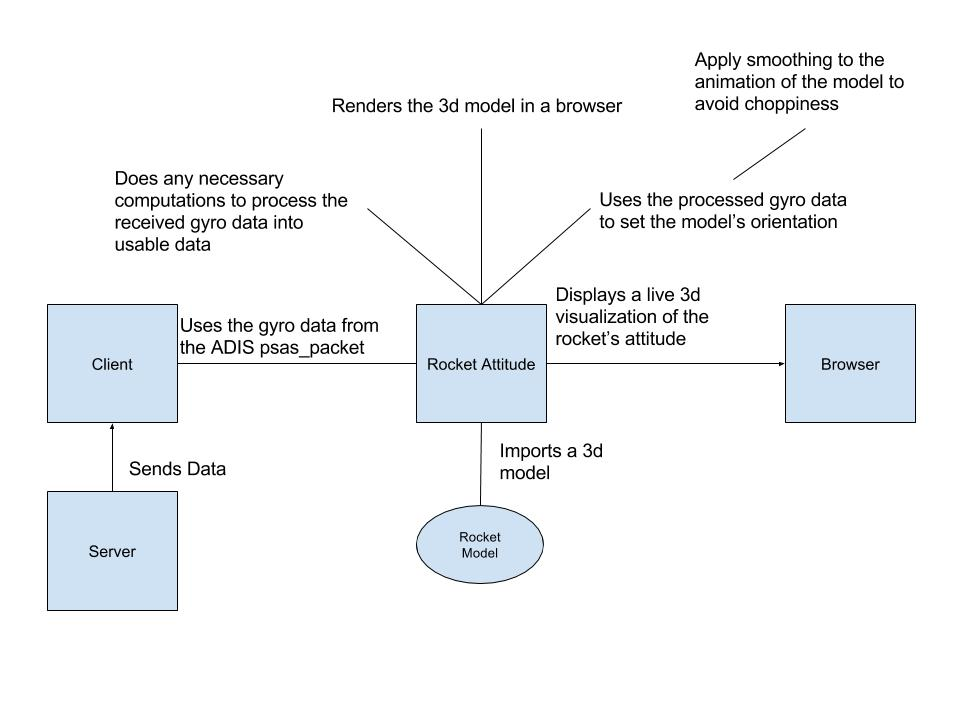
\includegraphics[scale=.4]{imgs/attitude.jpg}
\caption{Rocket Attitude \label{overflow}}
\end{figure}
